
\chapter{Introdução}
Tendo em vista a necessidade de aspiração em piscinas e a crescente onda de
automação residencial, observou-se a oportunidade de produzir um equipamento
para realizar tal tarefa automática de piscinas \cite{kanno2014}. 
Considerando o alto custo de aquisição de equipamentos modernos, internacionais
e a grande demanda por serviços de higienização de piscinas, e o fato de que no
Brasil não há empresas que desenvolvam este produto (há apenas revendedoras), o
desenvolvimento do \cpr permitirá a aplicação do conceito de automação
a ambientes residenciais e a redução dos gastos com a contratação de um serviço
terceirizado. As principais vantagens na utilização do \cpr são:
\begin{itemize}
\item Retirar detritos do fundo da piscina que não foram alcançados por outros meios;
\item Mover a água ao passo que limpa as superfícies, melhorando a sua circulação;
\item Produzir um produto nacional que possui valor de mercado mais acessível.
\end{itemize}

Por uma pesquisa realizada pela equipe, constatou-se que o peso dos robôs que limpam
piscinas varia de 8 Kg até 25 Kg e custam entre R\$ 2.000,00 e R\$ 16.000,00. Pequenas
diferenças de especificação devem ser consideradas no momento da aquisição do
aparelho, como por exemplo, ciclo de limpeza e taxa de filtragem. O ciclo de limpeza
determina o intervalo de tempo em que o robô trabalha antes de se desligar
automaticamente e a taxa de filtragem é determinada pela quantidade de água filtrada
em uma hora, que é expressa em litros por hora (LPH).

\section{Objetivos}
Construir um robô capaz de realizar a remoção de sujeiras depositadas no fundo de
piscinas por meio da aspiração e filtragem das impurezas. O objetivo específico
deste relatório é apresentar:
\begin{itemize}
\item O projeto de solução, modelagem, cálculos matemáticos e; 
\item As simulações; 
\item A Prototipagem das partes do robô e da solução.
\end{itemize}

\section{Estrutura do Relatório}
A organização do projeto foi dividido em dois grupos: o grupo de estrutura,
design e o grupo de lógica. Ambos os grupos se relacionam e tem trabalhado em
conjunto. O diagrama abaixo apresenta a interação entre os grupos e as diversas
engenharias que os compõem.
\par
\begin{figure}[h]
    \centering
    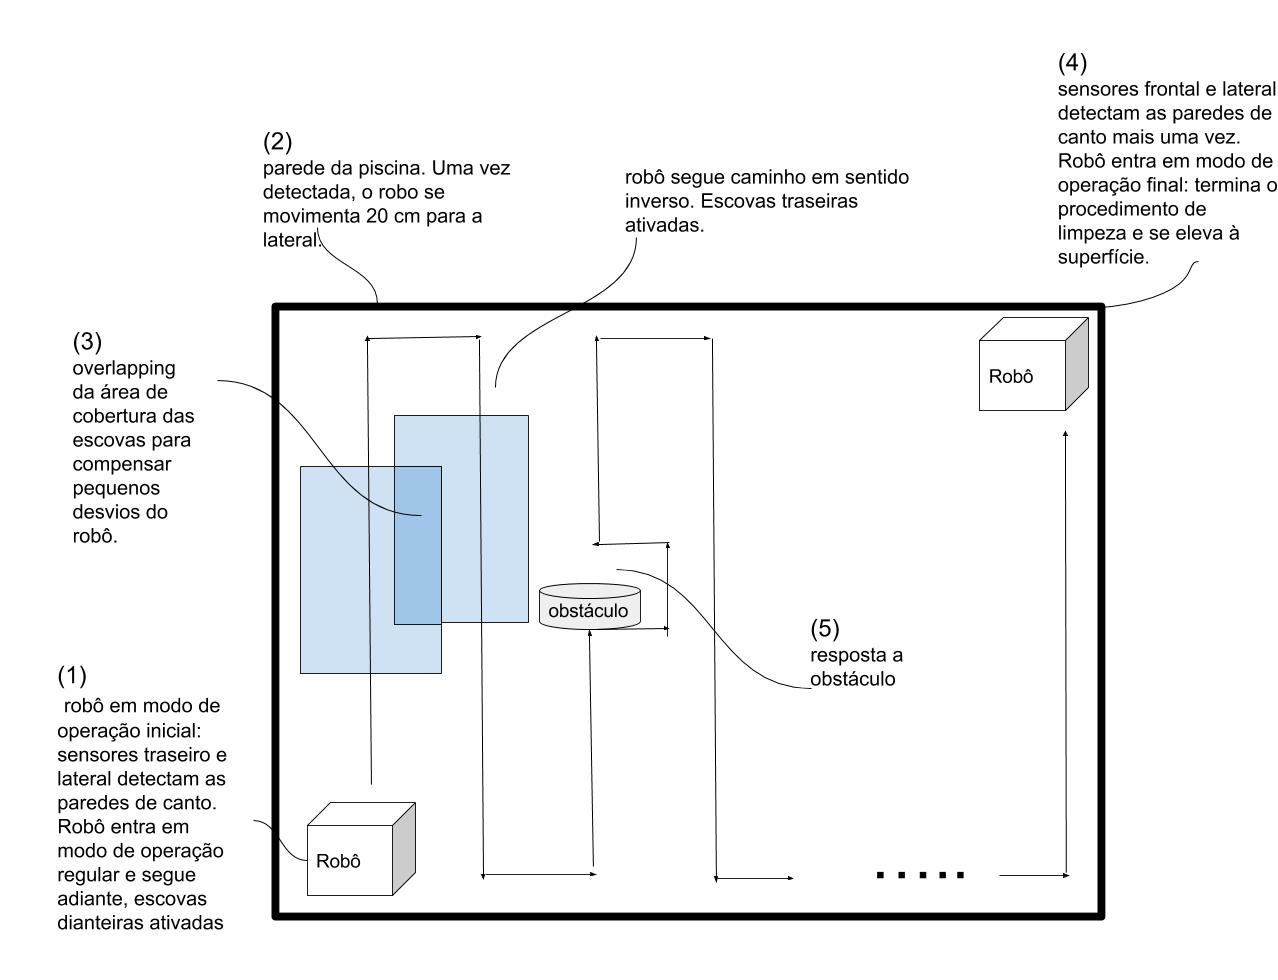
\includegraphics[width=\textwidth]{figures/schema-way-robot.jpg}
    \caption{Divisão técnica do projeto em dois segmentos (\textsf{Autoria do Autor})}
    \label{fig:technical-div-project}
  \end{figure}
\par
Apesar da divisão em duas grandes equipes, os membros interagiram de forma a
preencher os requisitos e parâmetros solicitados por meio de documentos compartilhados
via Google drive, ou por mensagens em grupos de conversa privados, utilizando-se do
WhatsApp.
Neste relatório estão apresentados na parte 2 a visão geral do robô, seu design,
sistemas, indicador e estimativa de custo. No Tópico 3 serão apresentados os sistemas
que compõem o \cpr, com o dimensionamento e cada componente. O Tópico 4
apresenta a montagem do protótipo do robô. O Tópico 5 demonstra os testes realizados
no protótipo.